\section{提案手法}

提案手法では、パラグラフベクトルによってレビュー内の各文及び文章の分散表現を
生成し、それらをニューラルネットワークの入力として分類を行う。
以下にその基礎となるアイデアと具体的なアルゴリズムを示す。


\subsection{アイデア}

先行研究\cite{fujitani15}の実験結果から、
レビュー内の文毎の素性を元にレビューの分類を行うことが
分類精度の向上に有効であると考えられる。
また、カテゴリ間の繋がりの変化が分類精度に影響していることから、
これをパラメータとして機械学習のモデルに組み込めば
分類精度を向上させることができると考えられる。
さらに、レビュー内の文毎に分散表現を生成し分類器の入力とすることで、
その順序を考慮した学習を行う。
これにより、レビュー内の文の位置関係がレーティング予測時に利用できる。

以下に、文の位置関係が重要となる例を示す。
2つ目の例は、1つ目の例の1つ目の文と3つ目の文を入れ替えたものである。
\begin{addmargin}{8ex}
  \vspace{1em}
  \setstretch{1}
  食事は本格的で新鮮な食材が使われており美味しかった。
  しかし、それよりも嬉しかったことがある。
  それは、部屋からの海の眺めが素晴らしかったことである。
  これには子供も喜んでいた。
\end{addmargin}
\begin{addmargin}{8ex}
  \vspace{1em}
  \setstretch{1}
  \textbf{それは、部屋からの海の眺めが素晴らしかったことである。}
  しかし、それよりも嬉しかったことがある。
  \textbf{食事は本格的で新鮮な食材が使われており美味しかった。}
  これには子供も喜んでいた。
\end{addmargin}
1つ目の例では、4つ目の文が直前の立地が良かったという文の
意味を補完しているのに対し、
2つ目の例では、食事が良かったという文の意味を補完している。
このように、文の位置関係によってどの文がどの文と強く関連しているかが変化する。
それによって、推定すべきレビュー全体のレーティングも変化すると考えられる。
よって、文の位置関係を考慮することは重要である。

しかし、個々のレビューに対して全ての文ベクトルを
ニューラルネットワークによる分類器の入力とすることは問題がある。
なぜならば、文の数はレビュー毎に異なっており、
複数レビュー内の複数の文ベクトルを単純な行列として表せないためである。
これは、分類器のミニバッチ方式の訓練を難しくし、
プログラムの実行時間を増加させる。
この問題に対処するため、本手法では各レビュー内の文ベクトルに対して
重み付け平均を行う。
これにより、全てのレビューで文ベクトルの数が揃い、
複数レビュー内の複数の文ベクトルをまとめて3次元行列として表すことができる。
つまり、ミニバッチ方式の計算が容易となる。

分類器はニューラルネットワークを用いて構成することによって、文の位置関係と
カテゴリ間の関係を同時に捉えた分類を行う。従来手法\cite{nal14}や
\cite{rie14}、\cite{duyu15}では、単語ベクトルに対して
畳込みニューラルネットワークが用いられている。
しかし、提案手法においては、畳み込みニューラルネットワークより
全結合ニューラルネットワークを用いた方が精度が高かったため、
分類器には後者のみを用いた。


\subsection{アルゴリズム}

提案手法の処理の流れを説明する。
図\ref{fig:MyAlgorithm}にアルゴリズム全体の概略を示す。

\begin{figure}
  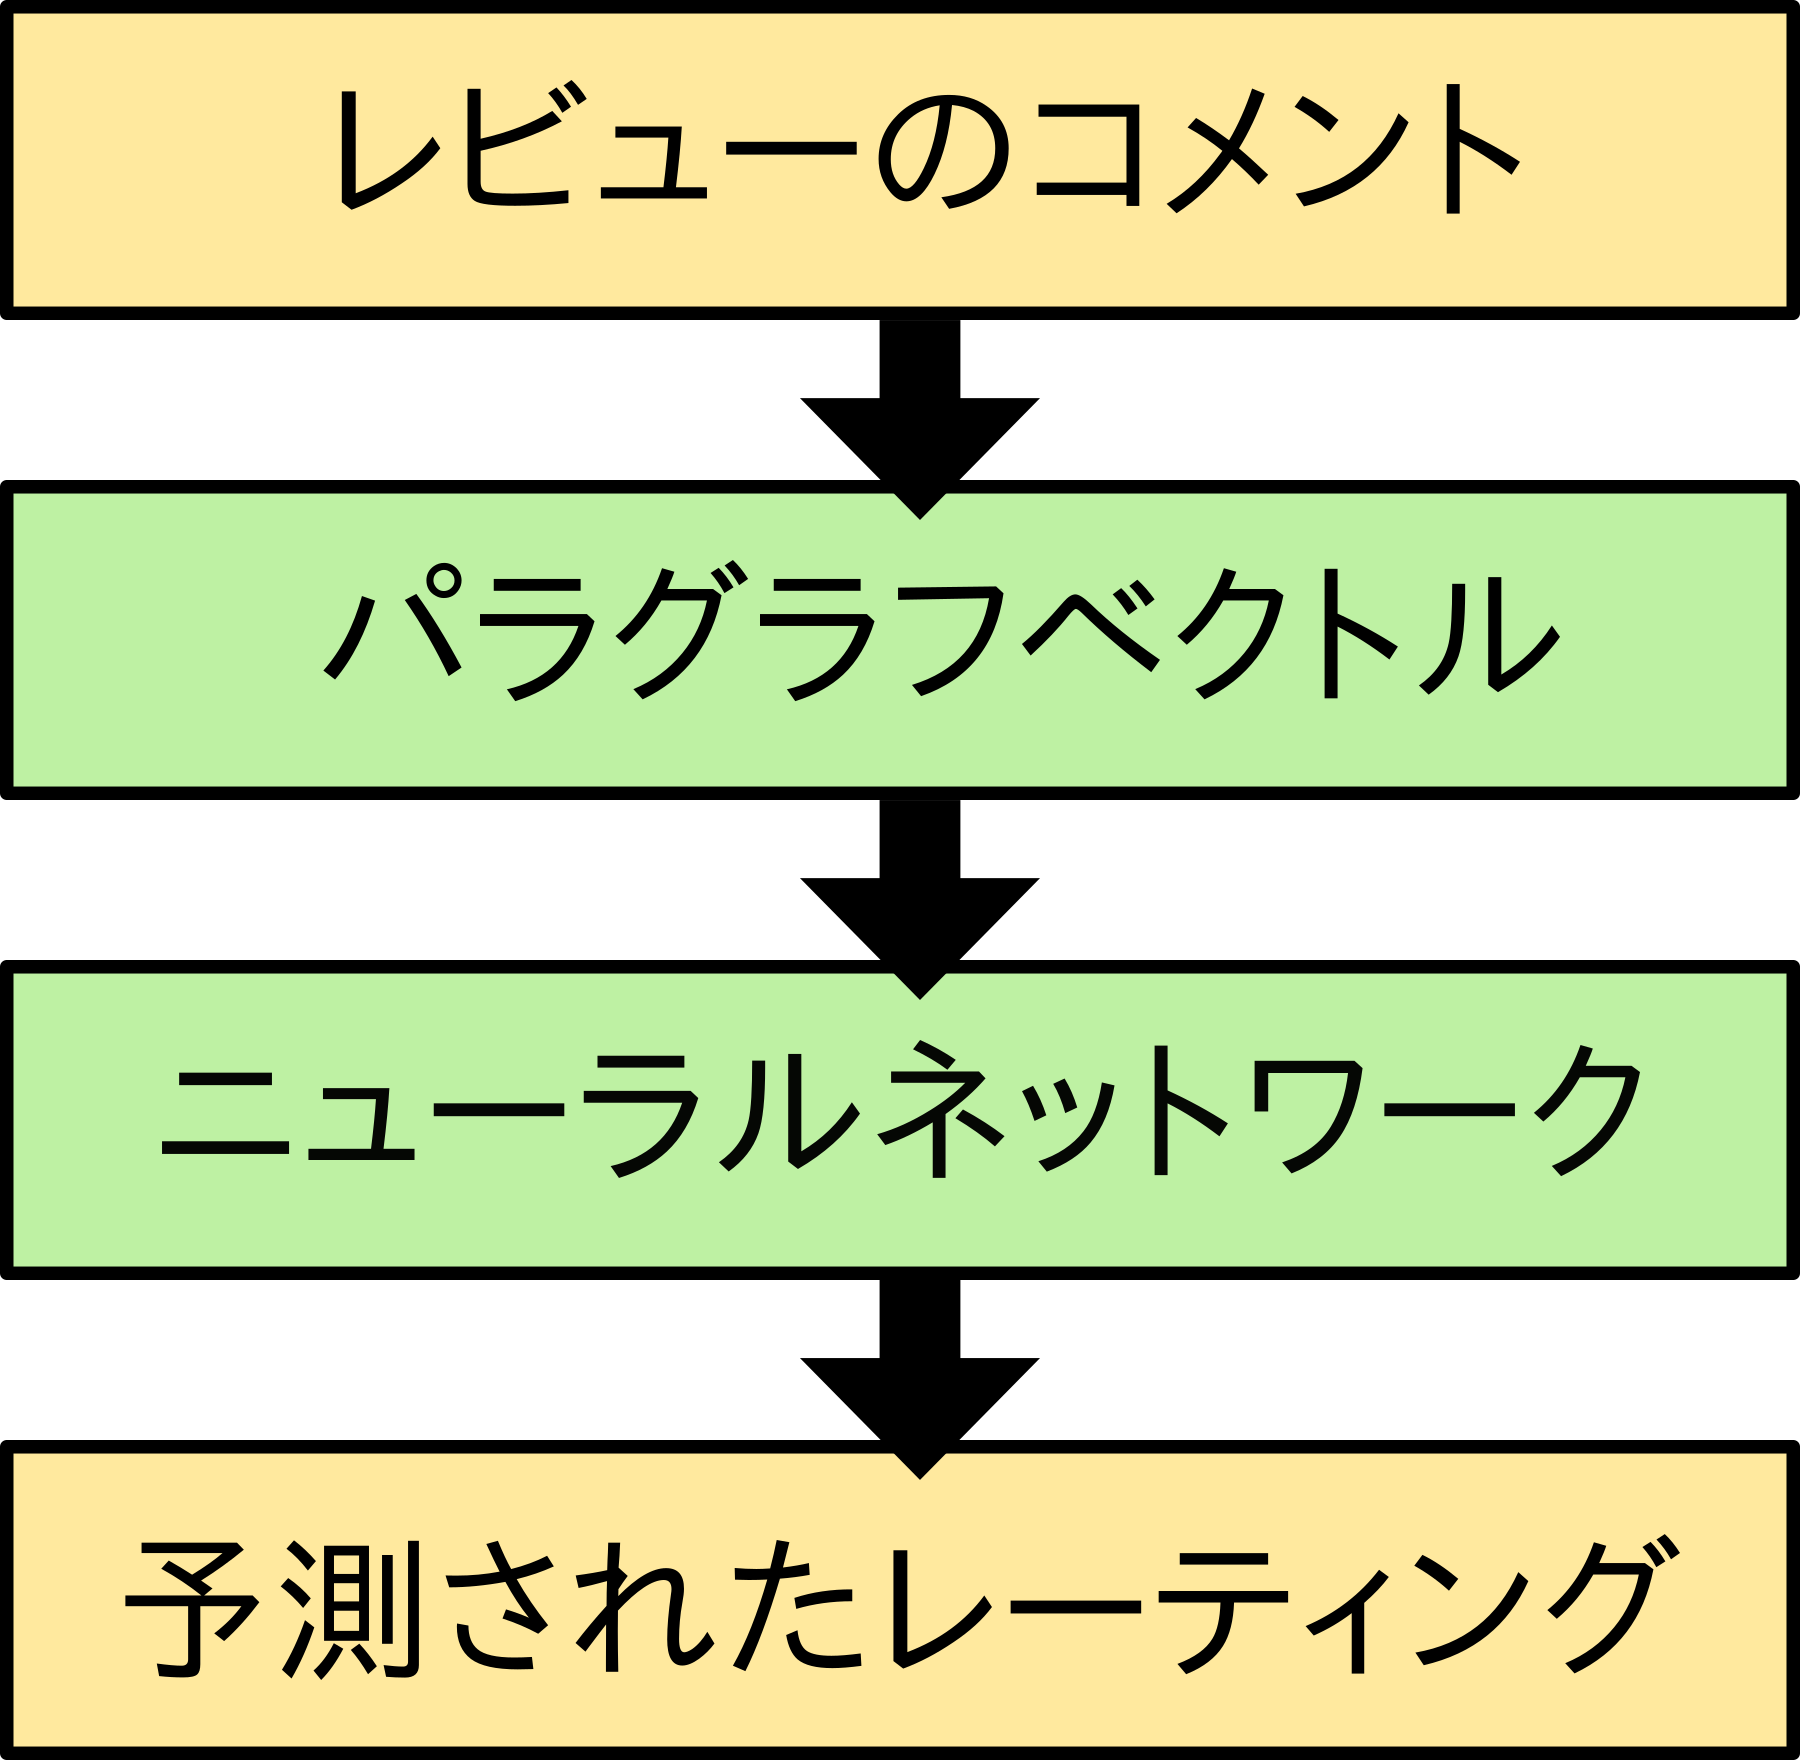
\includegraphics[0.5]{fig/algorithm.png}
  \caption{提案手法におけるアルゴリズムの概略}
  \label{fig:MyAlgorithm}
\end{figure}

%提案手法では、PV-DMによってレビュー内の文書全体及び各文の分散表現を
%生成し、それらをニューラルネットワークの入力として分類を行う。
%文毎の分散表現を用いることで文同士の位置関係を考慮し、
%ニューラルネットワークによる分類器を用いることで
%文間及びカテゴリ間の深い関係性を捉えることを目指す。
%提案手法の入力はレビューである文書と正解レーティングの組の集合、
%出力は各文書について予測されたカテゴリ毎のクラスである。
%以下に提案手法の処理の流れを示す。

初めに、PV-DMを用いて、
各レビューの文書ベクトルとそれに含まれる各文のベクトルを生成する。
文書ベクトルと文ベクトルについては別々に学習し生成する。
%式\ref{eq:PVObjective}に示す目的関数$L_d$を最大化するように学習を行う。
%\begin{multline}
%  L_d = \sum^{T}_{t = n + 1} \{ \log \sigma(s(w_t, w_{t-n}, ..., w_{t-1}, d)) \\
%        + \sum^{k}_{w_{t}' \sim P_n}
%        \log(1 - \sigma(s(w_{t}', w_{t-n}, ..., w_{t-1}, d))) \},
%    \label{eq:PVObjective} \\
%\end{multline}
%\begin{gather}
%  s(w_t, w_{t - n}, ..., w_{t - 1}, d)
%    = W_{map}(w_t)
%      \cdot \begin{bmatrix} W(w_{t - n}) \\ \vdots
%      \\ W(w_{t - 1}) \\ D(d) \end{bmatrix} \nonumber
%\end{gather}
%ここで、$T$は現在の文章内の単語数、$t$は現在の単語位置、$d$は現在の文章、
%$w_i$は位置$i$にある単語、$n$はウィンドウサイズである。
%$W(w_i)$は単語$w_i$に相当する単語ベクトルを単語行列$W$から抜き出す関数を表す。
%$D(d)$は文章$d$に相当する文章ベクトルを文章行列$D$から抜き出す関数を表す。
%関数$s(w_t, w_0, ..., w_n, d)$はある単語とそれが出現する文脈との類似度を
%計算する。
%行列$W_{map}$は内積によって文脈と単語との類似度を計算するための単語毎
%のベクトルを保持する。
%文章行列内の各文章ベクトルはレビュー全体を表す文書ベクトル、または、
%各レビュー内の文ベクトルを表す。
%$\sigma$はシグモイド関数である。
%また、式\ref{eq:PVObjective}の中括弧内の右項はネガティブサンプリングを
%表す。
%ネガティブサンプリングとは、文脈外の単語をデータセットにおける出現確率で
%サンプリングし、それらと文脈の意味が遠ざかるように学習する手法である。
%$w_{t}' \sim P_n$は文脈外の単語$w_{t}'$を単語の出現頻度$P_n$によって
%サンプリングすることを示す。
%ただし、出現頻度は極端に頻出する単語の影響を抑えるため
%各単語に対して3/4乗している。
%現在の単語と同じ単語や同一回の学習で一度サンプリングされた単語は
%サンプリングしない。
式\ref{eq:ParagraphVector}の目的関数における$h$には
引数のベクトルを結合する関数を用いる。
また、学習の高速化のため、Quocら\cite{quoc14}によって
用いられている階層的softmaxの代替として、ネガティブサンプリングを行う。
ネガティブサンプリングとは、文脈外の単語をデータセットにおける出現確率で
サンプリングし、それらと文脈の意味が遠ざかるように学習する手法である。
ただし、出現頻度は極端に頻出する単語の影響を抑えるため
各単語に対して3/4乗している。
現在の単語と同じ単語や同一回の学習で一度サンプリングされた単語は
サンプリングしない。

次に、各レビュー内の全ての文ベクトルに対して重み付け平均を行い、
圧縮された文ベクトルを生成する。
この過程により、各レビューで疎らだった文の数を統一する。
式\ref{eq:WeightedAverageSV}に重み付け平均によって圧縮した
文ベクトル$t_{i_{part}}$を示す。
各文ベクトルは圧縮後の各文ベクトルと位置が近いほど重みが大きくなるように
重み付け平均する。
\begin{gather}
  \mathbf{t}_{i_{part}} = \sum_{i_{sent}}
                          \frac{w(x_{i_{part}}(i_{sent}))}
                               {|\sum_{i_{sent}'} w(x_{i_{part}}(i_{sent}'))|}
                          \mathbf{s}_{i_{sent}},
  \label{eq:WeightedAverageSV} \\
  x_{i_{part}}(i_{sent}) = \frac{i_{sent} - i_{part}}{\#partitions},
  \nonumber \\
  w(x) = \begin{cases}
    \frac{1}{2} (\cos(\pi|x|) + 1) &\text{if $|x| <= 1$} \\
    0 &\text{otherwise}
  \end{cases} \nonumber
\end{gather}
ここで、$i_{sent}$はレビュー内の文のインデックス、
$\#partitions$は重み付け平均された後の文ベクトルの数、
$i_{part}$は重み付け平均された後の文ベクトルのインデックス、
$\mathbf{s}_{i_{sent}}$は文ベクトルである。
\footnote{重み付けの関数には$\cos$関数の他に、
$x$に対して線形に重みを減少させるような関数や、
単純に文を区画毎に平均するような関数も考えられる。
区画毎に平均する関数は他の2つより正答率が低く、線形な関数と
$\cos$関数はほぼ同じ正答率を示したため、$\cos$関数を採用した。}

最後に、分類器によってレーティング予測を行う。
分類器は全結合ニューラルネットワークによって構成される。
図\ref{fig:MyModel}に各層の結合の様子を示す。
\begin{figure}[t!]
  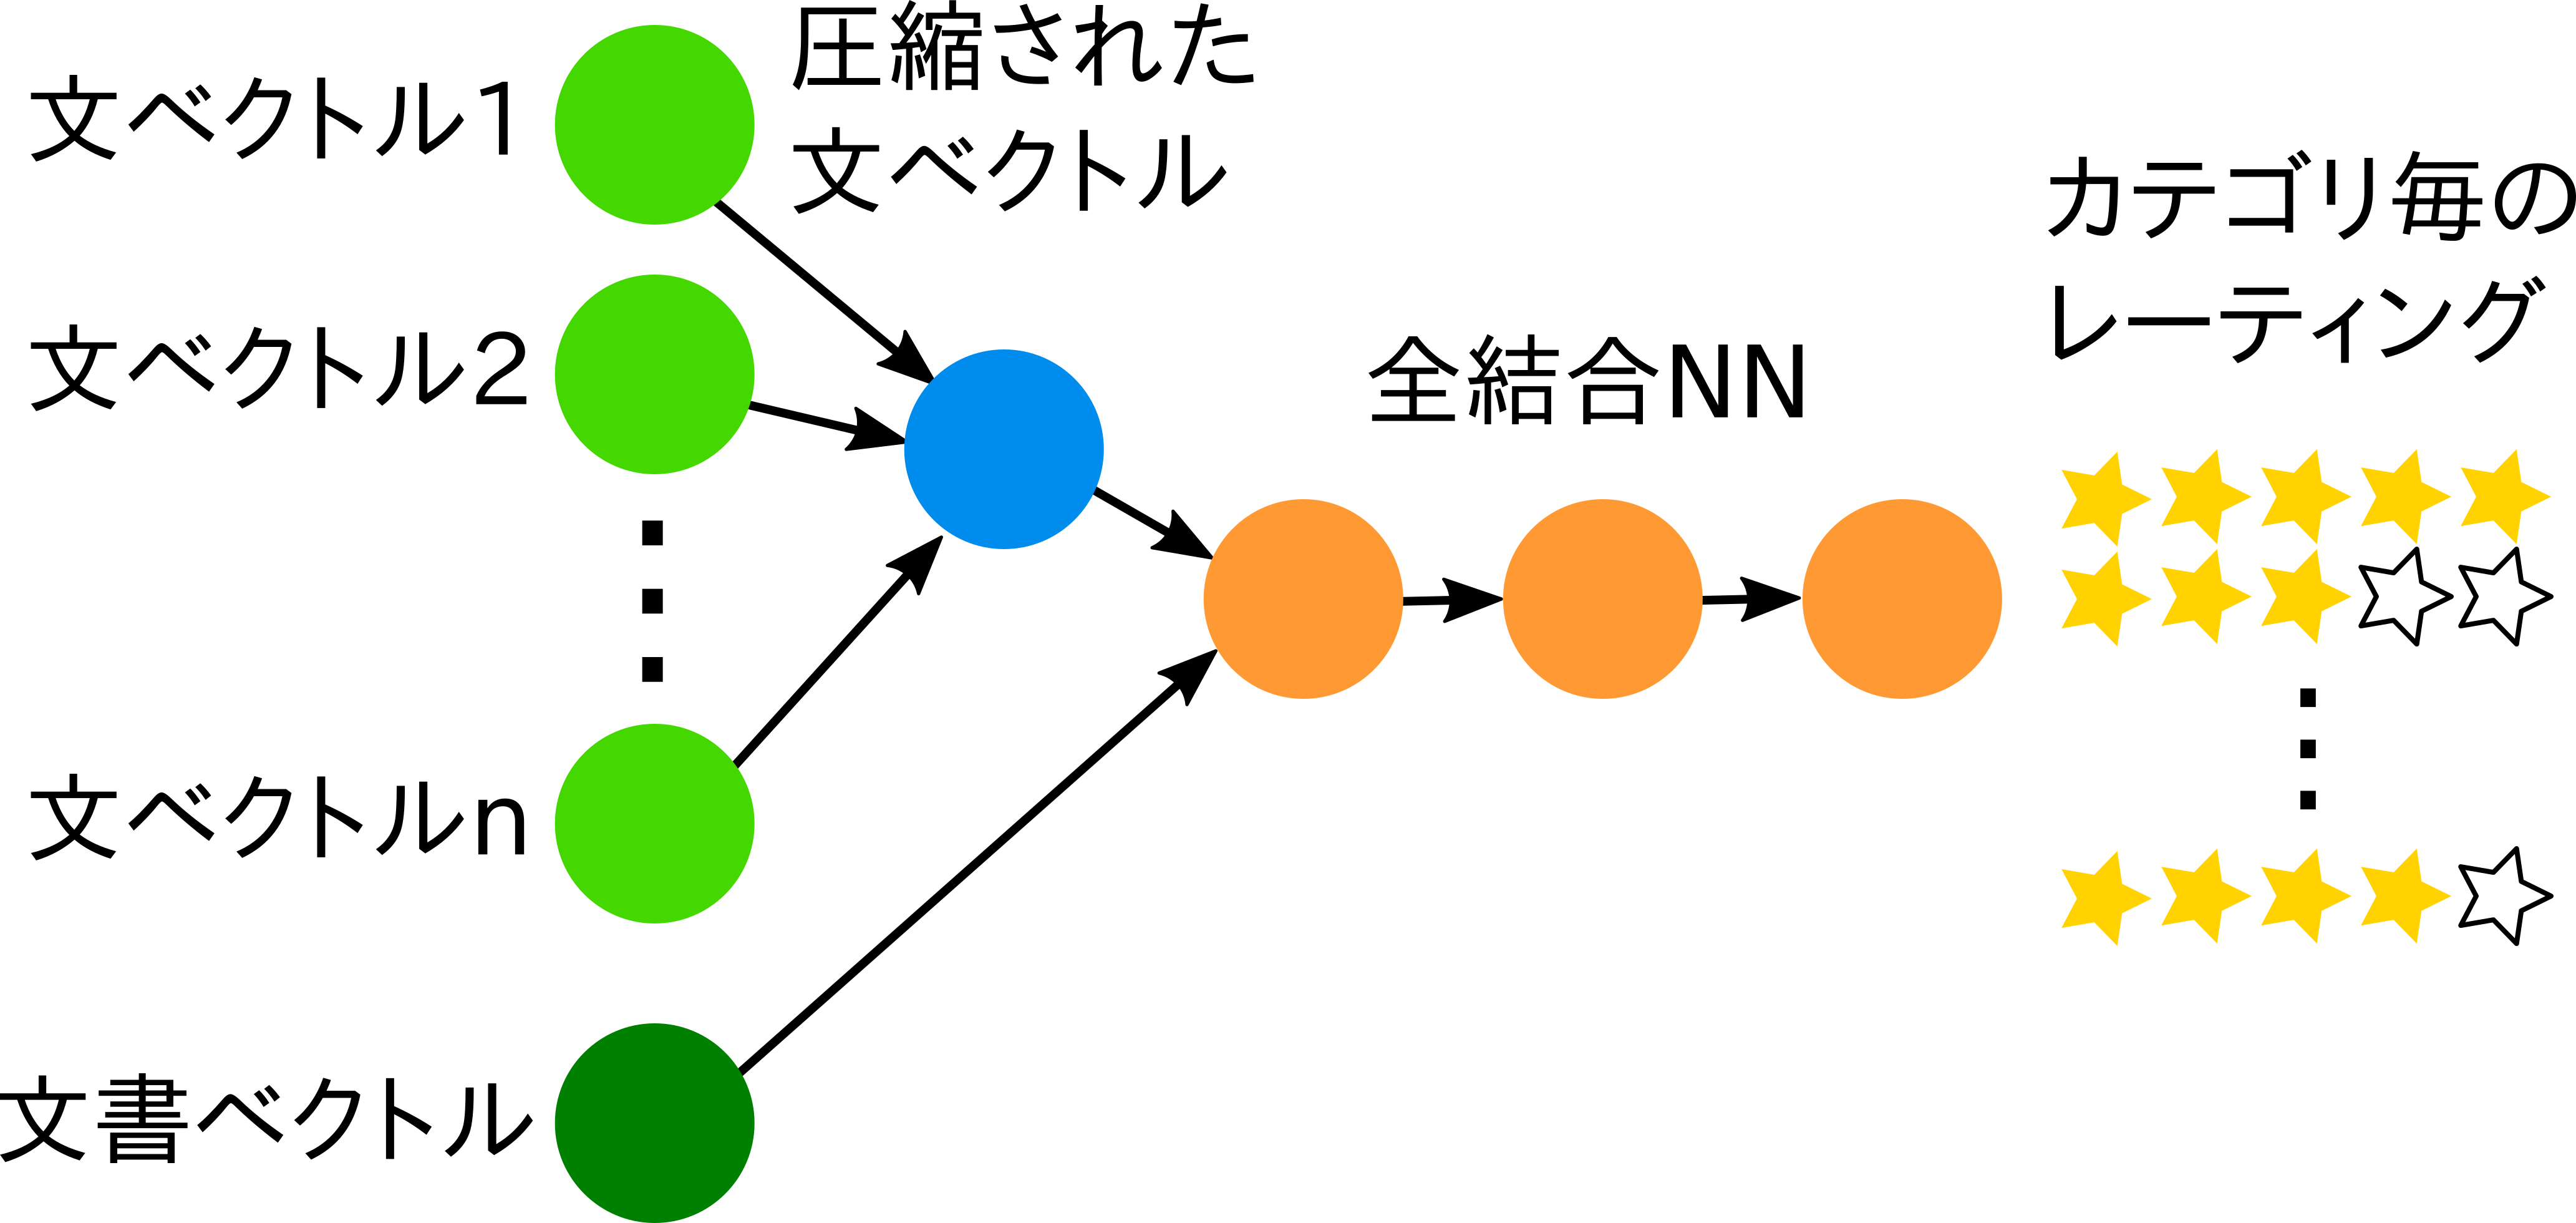
\includegraphics{fig/model.png}
  \caption{全結合ニューラルネットワークによる分類器}
  \label{fig:MyModel}
\end{figure}
入力層はレビュー毎の文書ベクトルと圧縮された文ベクトルの結合ベクトルである。
ニューラルネットワークの活性化関数には、シグモイド関数を用いる。
また、出力層はカテゴリの数とラベルの数の積だけのユニットを持ち、
各ユニットの出力はあるカテゴリ内であるクラスが選ばれることの
正規化されていない対数確率を表す。
ニューラルネットワークは式\ref{eq:NNObjective}に示す目的関数$E$を
最小化するように学習を行う。
\begin{gather}
  E = - \sum^{N}_{n = 1} \sum^{C}_{c = 1} \sum^{K}_{k = 1}
        d_{nck} \log{y_{ck}(x_n; w)},
  \label{eq:NNObjective} \\
  y_{ck}(x_n; w) = \frac{e^{u_{ck}(x_n; w)}}
                        {\sum^{K}_{j = 1} e^{u_{cj}(x_n; w)}} \nonumber
\end{gather}
各ユニットの出力はカテゴリ毎に交差エントロピー誤差関数によって
損失に変換される。
ここで、$u_{ck}$は出力層のユニットの出力値、$y_{ck}$はカテゴリ$c$において
クラス$k$が選ばれる確率、$w$はニューラルネットワークのパラメータである。
$d_{nck}$は$n$番目の文書がカテゴリ$c$でクラス$k$ならば1、
それ以外で0となる値である。
$N$はミニバッチサイズ、$C$はカテゴリの総数、$K$はクラスの総数である。
